% \section{Legendre Memory Units}
% \label{sec:nlp_lmu}

\section{Efficiently Modeling Long Sequences with Structured State-Spaces}
\label{sec:nlp_ssm}
The Linear State-Space Layer (LSSL) is a simple sequence model that maps a one-dimensional function  or sequence $u(t)\to y(t)$ through an implicit state $x(t)$ by simulating a linear continuous-time state-space representation in discrete-time
\begin{align*}
	x'(t) &= \mathbf{A}x(t)+\mathbf{B}u(t),\\
	y(t) &= \mathbf{C}x(t)+\mathbf{D}u(t).
\end{align*}

The first equation maps a single dimensional input signal $u(t)$ (or sequence) to an $N$-dim latent state (or hidden state) $x'(t)$ with the current state $x(t)$. The $\mathbf{A}$ and $\mathbf{B}$ can be considered as an non-linear mapping or transition matrices (\ie learnable parameters) to reflect the impact of the current state and the input, respectively. Finally, we project the input and the updated state to a one-dim output signal $y(t)$ (\ie sequence).  

Our goal is to simply use the SSM as a black-box representation in a deep sequence model, where $\rmA, \rmB, \rmC$, and $\rmD$ are parameters learned by gradient descent. We will omit the parameter $\rmD$ for exposition (or equivalently, assume $\rmD=0$, because the term $\rmD u$ can be viewed as a \textit{skip connection} that doesn't depend on the hidden state ($x$)).

An SSM maps a input $u(t)$ to a state representation vector $x(t)$ and an output $y(t)$. For simplicity, we assume the input and output are one-dimensional, and the state representation is $N$-dimensional. The first equation defines the change in $x(t)$ over time.

\begin{figure}[t]
	\centering
	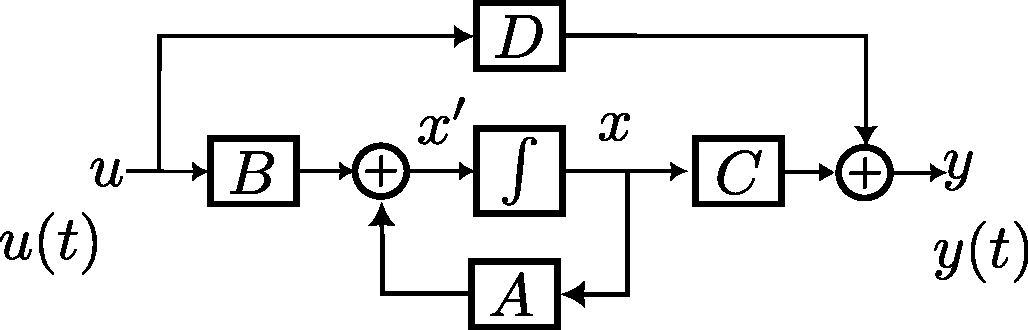
\includegraphics[scale=0.6]{./images/nlp/ssm.pdf}
	\caption{S4 Model}
	\label{fig:nlp_s4_model}
\end{figure}

\paragraph{Discretization} We want to find a discrete-time state-space model. We can represent it by approximating a continuous model (\ie $h(t_k) \approx h(k\Delta)$) as follows:
\begin{align*}
	x'(t) &= \overline{\mathbf{A}}x(t)+\overline{\mathbf{B}}u(t),\\
	y(t) &= \mathbf{C}x(t)+\underbrace{\mathbf{D}u(t)}_{=0},
\end{align*}
where $\overline{\mathbf{A}} = \mathbf{I}+\Delta \mathbf{A}$ and $\overline{\mathbf{B}} = \Delta \mathbf{B}$, respectively. They are derived by
\begin{align*}
	x'(t) &= \overline{\mathbf{A}}x(t)+\overline{\mathbf{B}}u(t)\\
		  &= \lim_{\Delta\to 0} \frac{x(t+\Delta)-x(t)}{\Delta},
\end{align*}
where $\Delta$ is a step size. Note that $\Delta$ is a learnable parameter to be determined during a training phase. Subsequently, we get 
\begin{align*}
	x(t+\Delta)-x(t) = \Delta x'(t).
\end{align*}
Equivalently, 
\begin{align*}
	x(t+\Delta) = \Delta x'(t)+x(t). 
\end{align*}
Plugging $x'(t)$ into the above equation, we get:
\begin{align*}
	x(t+\Delta) &= \Delta (\mathbf{A}x(t)+\mathbf{B}u(t)) +x(t) \\
				&= \underbrace{(\mathbf{I}+\Delta \mathbf{A})}_{\overline{\mathbf{A}}}x(t)+\underbrace{\Delta \mathbf{B}}_{\overline{\mathbf{B}}}u(t).
\end{align*}
We can say $x(t+\Delta)=x(t+1)$, since it is the next state we care. Thus, 
\begin{align*}
	x(t+1)= (\mathbf{I}+\Delta \mathbf{A})x(t)+\Delta \mathbf{B}u(t).
\end{align*}
Note that the original paper utilizes a special rule called \textit{Zero-Order Hold} to approximate the $\overline{A}$ and $\overline{B}$. 

Alternatively, we can use the trapezoidal method. The trapezoidal rule works by approximating the region under the graph of the function $f(x)$ as a trapezoid and calculating its area. It follows that
$$\int _{a}^{b}f(x)\,dx\approx (b-a)\cdot {\tfrac {1}{2}}(f(a)+f(b)).$$
Thus, the integral of $x'(t)$ from $t_n$ to $t_{n+1}$ can be approximated using the trapezoidal rule. The exact integral is:
\begin{align*}
	x(t_{n+1})-x(t_n) &= \int_{t_n}^{t_{n+1}}x'(t)dt\\
					  &\approx \frac{1}{2}\Delta (\mathbf{A}x(t_{n+1})+\mathbf{B}u(t_{n+1})+\mathbf{A}x(t_n) + \mathbf{B}u(t_n)),
\end{align*}
where $\Delta = t_{n+1}-t_n$. Then, we have 
\[ x(t_{n+1}) - \frac{\Delta}{2} \mathbf{A}x(t_{n+1}) = x(t_n) + \frac{\Delta}{2} \mathbf{A}x(t_n) + \frac{\Delta}{2} \mathbf{B}u(t_n) + \frac{\Delta}{2} \mathbf{B}u(t_{n+1}) \]

\[ \bigg(\mathbf{I} - \frac{\Delta}{2} \mathbf{A}\bigg) x(t_{n+1}) = \bigg(\mathbf{I} - \frac{\Delta}{2} \mathbf{A}\bigg) x(t_n) + \Delta \mathbf{B} \frac{(u(t_n) + u(t_{n+1})}{2} \]

\[ x(t_{n+1}) = \left( \mathbf{I} - \frac{\Delta}{2} \mathbf{A} \right)^{-1} \left( \mathbf{I} + \frac{\Delta}{2} \mathbf{A} \right) x(t_n) + \left( \mathbf{I} - \frac{\Delta}{2} \mathbf{A} \right)^{-1} \frac{\Delta}{2} \mathbf{B} (u(t_{n+1})) \]
Finally, we get
\begin{align*}
	\overline{\mathbf{A}} &= \left( \mathbf{I} - \frac{\Delta}{2} \mathbf{A} \right)^{-1} \left( \mathbf{I} + \frac{\Delta}{2} \mathbf{A} \right)\\
	\overline{\mathbf{B}} &= \left( \mathbf{I} - \frac{\Delta}{2} \mathbf{A} \right)^{-1} \Delta \mathbf{B}
\end{align*}
Note that we assume that $u(t_{n+1})\approx u(t_{n}).$ We can represent the update process as follows:
At $t=0$
\begin{align*}
	x(0) &= \overline{\mathbf{B}}u(0),\\
	y(0) &= \mathbf{C}x(0)
\end{align*}

At $t=1$
\begin{align*}
	x(1) &= \overline{\mathbf{A}}x(0)+\overline{\mathbf{B}}u(1),\\
	y(1) &= \mathbf{C}x(1)
\end{align*}

At $t=2$
\begin{align*}
	x(2) &= \overline{\mathbf{A}}x(1)+\overline{\mathbf{B}}u(2),\\
	y(2) &= \mathbf{C}x(2).
\end{align*}
Note that this update process is equivalent to the RNN's update process. 

\paragraph{As a Convolution} 
The above process can be viewed as an one-dimensional convolution. 

\begin{align*}
	x(0) &= \overline{\mathbf{B}}u(0),\\
	y(0) &= \mathbf{C}x(0) = \mathbf{C}\overline{\mathbf{B}}u(0)\\
		 &\\
	x(1) &= \overline{\mathbf{A}}x(0)+\overline{\mathbf{B}}u(1)=\overline{\mathbf{A}}\overline{\mathbf{B}}u(0)+\overline{\mathbf{B}}u(1)\\
	y(1) &= \mathbf{C}x(1) = \mathbf{C}(\overline{\mathbf{A}}\overline{\mathbf{B}}u(0)+\overline{\mathbf{B}}u(1)) = \mathbf{C}\overline{\mathbf{A}}\overline{\mathbf{B}}u(0)+\mathbf{C}\overline{\mathbf{B}}u(1)\\
		 &\\
	x(2) &= \overline{\mathbf{A}}x(1)+\overline{\mathbf{B}}u(2)=\overline{\mathbf{A}}(\overline{\mathbf{A}}\overline{\mathbf{B}}u(0)+\overline{\mathbf{B}}u(1))+\overline{\mathbf{B}}u(2)=\overline{\mathbf{A}}^2\overline{\mathbf{B}}u(0)+\overline{\mathbf{A}}\overline{\mathbf{B}}u(1)+\overline{\mathbf{B}}u(2)\\
	y(2) &= \mathbf{C}x(2)=\mathbf{C}(\overline{\mathbf{A}}^2\overline{\mathbf{B}}u(0)+\overline{\mathbf{A}}\overline{\mathbf{B}}u(1)+\overline{\mathbf{B}}u(2))=\mathbf{C}\overline{\mathbf{A}}^2\overline{\mathbf{B}}u(0)+\mathbf{C}\overline{\mathbf{A}}\overline{\mathbf{B}}u(1)+\mathbf{C}\overline{\mathbf{B}}u(2)\\
\end{align*}
We get a general formula:
\begin{align*}
	y(t) &= \mathbf{C}\overline{\mathbf{A}}^t\overline{\mathbf{B}}u(0)+\mathbf{C}\overline{\mathbf{A}}^{t-1}\overline{\mathbf{B}}u(1)+\dots+\mathbf{C}\overline{\mathbf{B}}u(t)\\
		 &= \sum_{t=0}^T \mathbf{C}\overline{\mathbf{A}}^{T-t}\overline{\mathbf{B}}u(t)
\end{align*}
It turns out that the above equation is a one-dimensional convolution by a kernel $\overline{\mathbf{K}}$:
\begin{align*}
	y = x*\overline{\mathbf{K}}.
\end{align*}
It is generally referred to as the SSM convolution kernel in the literature, and its size is equivalent to the entire input sequence. This convolution kernel is calculated by Fast Fourier Transform (FFT)

\begin{figure}[t]
	\centering
	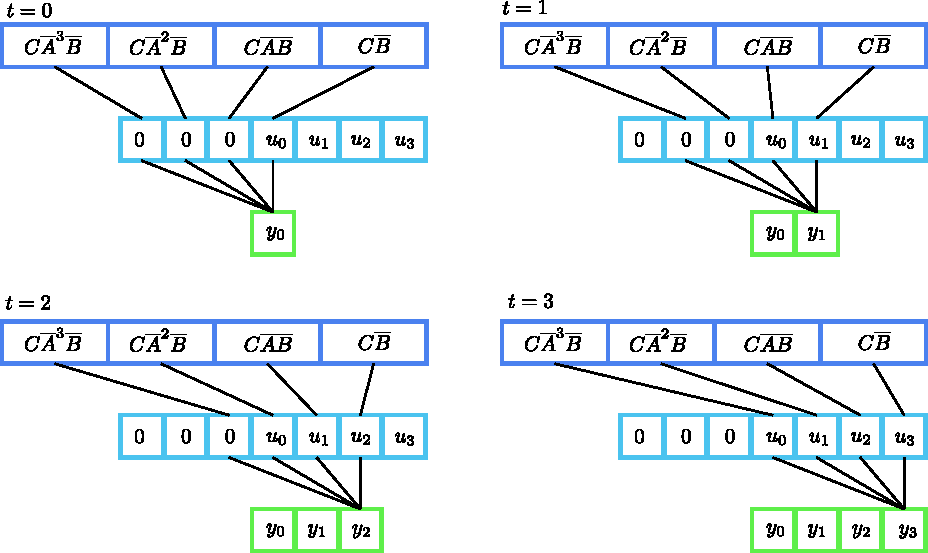
\includegraphics[scale=0.95]{./images/state_space/mamba_conv.pdf}
	\caption{}
	\label{fig:mamba_conv}
\end{figure}

Let's say the kernel size is 4 with zero-padding,  (See \Cref{fig:mamba_conv}). During training, we can train the model as a convolutional neural network so that we can leverage the parallel training. During inference (\ie decoding stage), we can switch to the recurrent mode for near-constant time inference. Please note here, that if you look at the kernels you can see that they are fixed. 


In the convolution kernel developed above, $\mathbf{\bar{C}}$ and $\mathbf{\bar{B}}$, are learnable scalars.
Concerning $\mathbf{\bar{A}}$, we've seen that in our convolution kernel, it's expressed as a power of $k$ at time $k$. This can be very time-consuming to calculate, so we're looking for a fixed $\mathbf{\bar{A}}$. For this, the best option is to have it diagonal:


Note that we can scale the single-dimensional SSM to multi-dimensional vector by putting a SSM for each dimension. For instance, there is going to be 256 SSMs if we want to learn a 256 embeddings.  


\section{Mamba: Linear-Time Sequence Modeling with Selective State Spaces}
\label{sec:ssm_mamba}
https://blog.premai.io/s4-and-mamba/

We can immediately notice the importance of the matrix $\mathbf{A}$. The Mamba leverages a special matrix called HiPPO. The HiPPO is a $N x N$ matrix specifically designed to approximate all the input signals by using Legendre polynomials (like Fourier series). 
\begin{align*}
	\mathbf{A}_{nk} = 
\begin{cases}
	(2n+1)^{1/2}(2k+1)^{1/2}\, &\textrm{ if } n>k\\
	n+1\, &\textrm{ if } n=k\\
	0\, &\textrm{ else }
\end{cases}
\end{align*}
This matrix helps to compress the history of the information by masking the next tokens, which is similar to the masked self-attention. Note that the matrix just needs to be computed once. 


